%%%%%%%%%%%%%%%%%%%%%%%%%%%%%%%% 
\section{The DCS, DSS} 
\label{sec:detectors-fd-alt-dcs}

The slow control system for the far detector is part of a continued progressive prototyping effort aiming at developing a control system dedicated to multi-ton liquid argon double phase detectors. It has been designed in the framework of the LAGUNA-LBNO design study and of the WA105 experiment following the successful example and the expertise developed in the context of the ArDM experiment  \cite{Badertscher:2013ygt}. ArDM  is currently operating 1 ton of liquid argon in an underground laboratory (LSC, Spain).  This slow control system is introducing for the first time the use of National Instruments compact RIO modules for acquisition of all the physical quantities of interest. In Figure~\ref{fig:NI_proto} a rack prepared for the WA105  $3 \times 1 \times 1$ $m^3$ prototype and ready to be tested at CERN is shown.

The slow control system of the far detector and $3 \times 1 \times 1$ $m^3$ prototype detectors is designed to monitor inside the tank the following physical quantities:

\begin{itemize}
  \item temperatures through platinum resistors,
  \item pressures with commercial piezoelectric sensors,
  \item liquid argon levels with custom made capacitive sensors and electronics,
  \item deformations of materials with resistive strain gauges
\end{itemize} 

Moreover, the slow control system  provides the hardware infrastructure needed to monitor traces of O2, N2 and H2O impurities in the tank, to monitor and control the high and low voltage power supplies, heaters, lighting system and cryogenic cameras video system. It will also interface to the cryogenic system and to the motorized system to adjust the position of each CRP. 

\begin{cdrfigure}[Slow Control prototype rack]{NI_proto}{The rack is a prototype of the entire Control System; it  embeds modules for resistive temperature sensors, pressure  sensors, strain gauges, liquid argon level meters, control for  heaters. On the upper part a redundant 24 V power supply provides
 fault tolerant power to the National Instrument controller and modules. Calibration of modules and sensors is ongoing.}
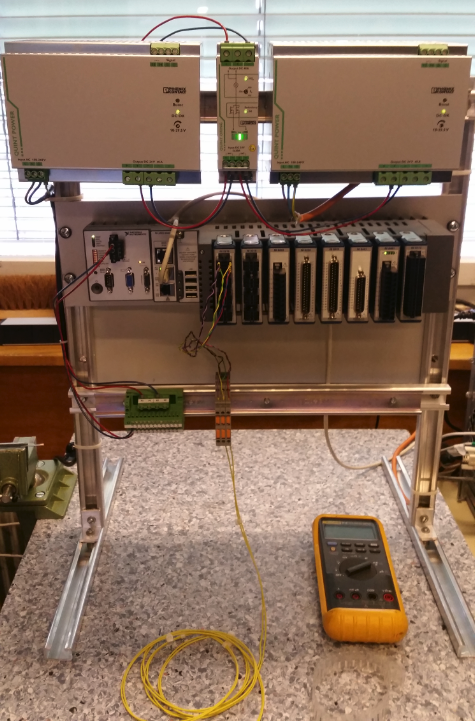
\includegraphics[scale=0.4, angle=0]{rack_2.jpg}
\end{cdrfigure}

The entire slow control system of the WA105 demonstrator will be managed through a single LabView  interface which will provide access to all the sensors, control the actuators and provide the platform for the video-cameras monitoring system inside and outside the tank.  The overlying supervisory level  will be implemented in UNICOS and it will provide the operator interface for the monitoring of all the physical quantities and the handling of alarms, as commonly done in CERN experiments.  

As already detailed in Section~\ref{sec:detectors-fd-ref-ov}, the charge readout system of the far detector is implemented in CRP modules of 3$\times$3 m$^2$. Each 3$\times$3 m$^2$ CRP is an independent detector, hence its instrumentation can be thought independently too. A complete list of the sensors which are been foreseen for both the 3$\times$3 m$^2$ far detector module and $3 \times 1 \times 1$ $m^3$ WA105 prototype  is provided in Table~\ref{fig:sc_sensors}. The number of sensors presented for the far detector CRP is  based on the extrapolation of the sensors foreseen the $3 \times 1 \times 1$ $m^3$ prototype and it is not yet final.  The sensors instrumentation of the $3 \times 1 \times 1$ $m^3$ WA105 prototype  has also led to the design of a custom made Slow Control feedthroughs (SCFT), based on the use of weldable connectors for High Vacuum (Figure~\ref{fig:SC_flange}). A specific Slow Control feedthrough for the 3$\times$3 m$^2$ CRP of the DUNE far detector is foreseen on the basis of this design.

\begin{cdrfigure}[Slow control feedthroughs]{SC_flange}{The 3 SCFTs providing weldable connectors for all the instrumentation inside the  $3 \times 1 \times 1$ $m^3$  WA105 tank. The number of sensors per module in the DUNE far detector will be drastically reduced with respect to this WA105 prototype.}
  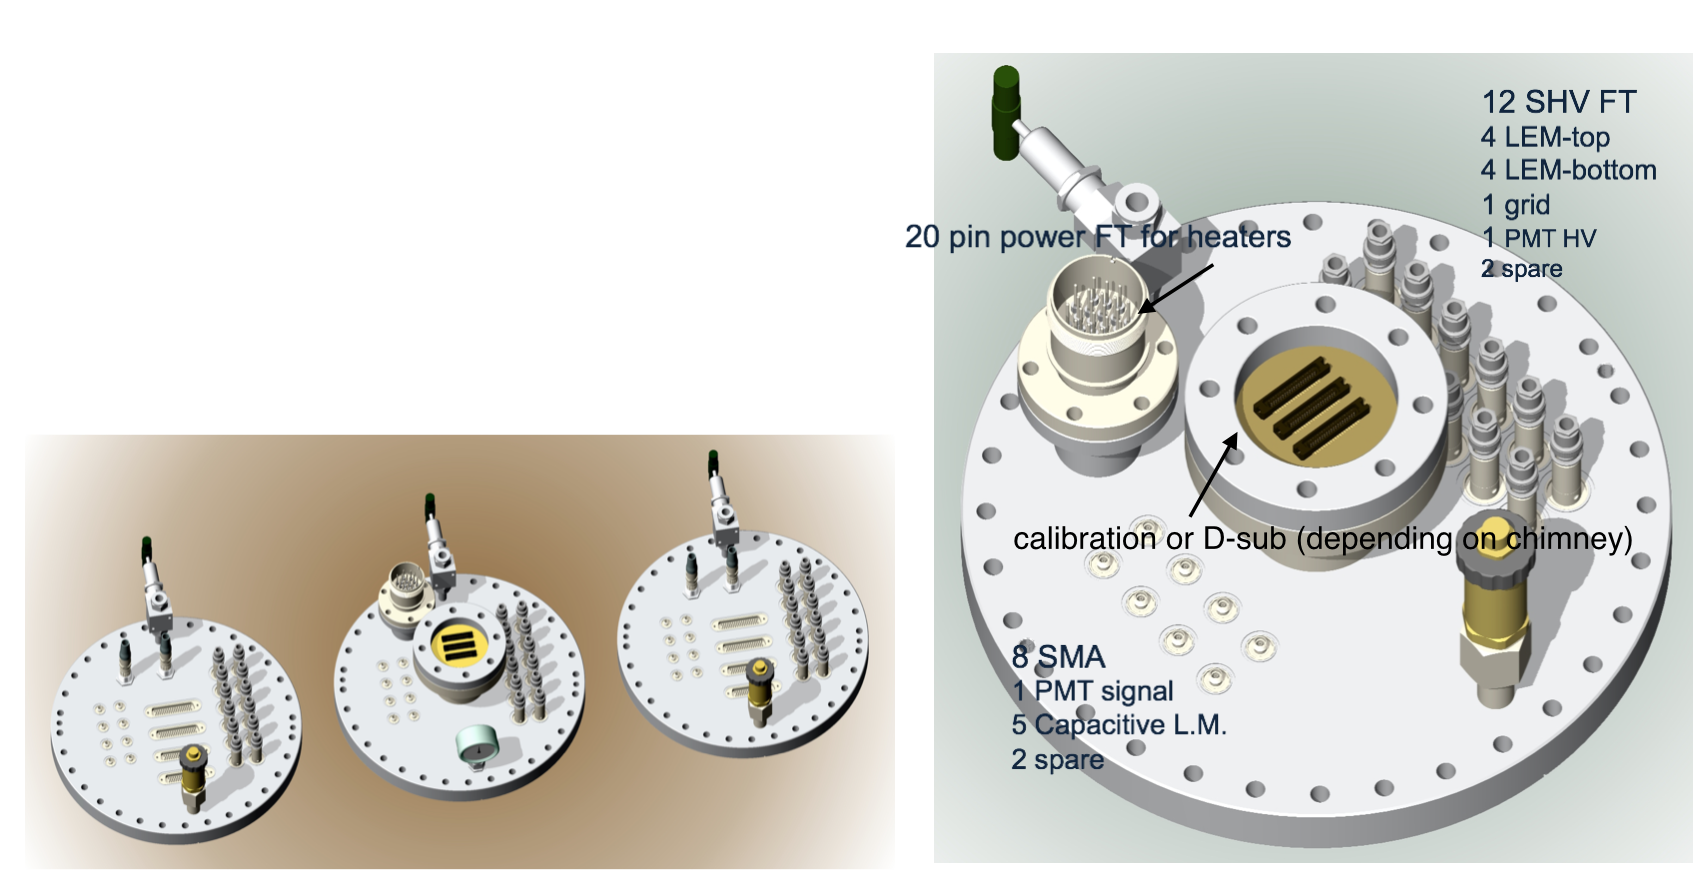
\includegraphics[scale=0.52, angle=0]{SC_flange.png}
 \end{cdrfigure}

\begin{cdrfigure}[List of the slow control sensors for  the $3 \times 1 \times 1$ $m^3$ prototype and far detector detectors.]{sc_sensors}{List of the slow control sensors for the $3 \times 1 \times 1$ $m^3$ prototype and far detectors CRP}
 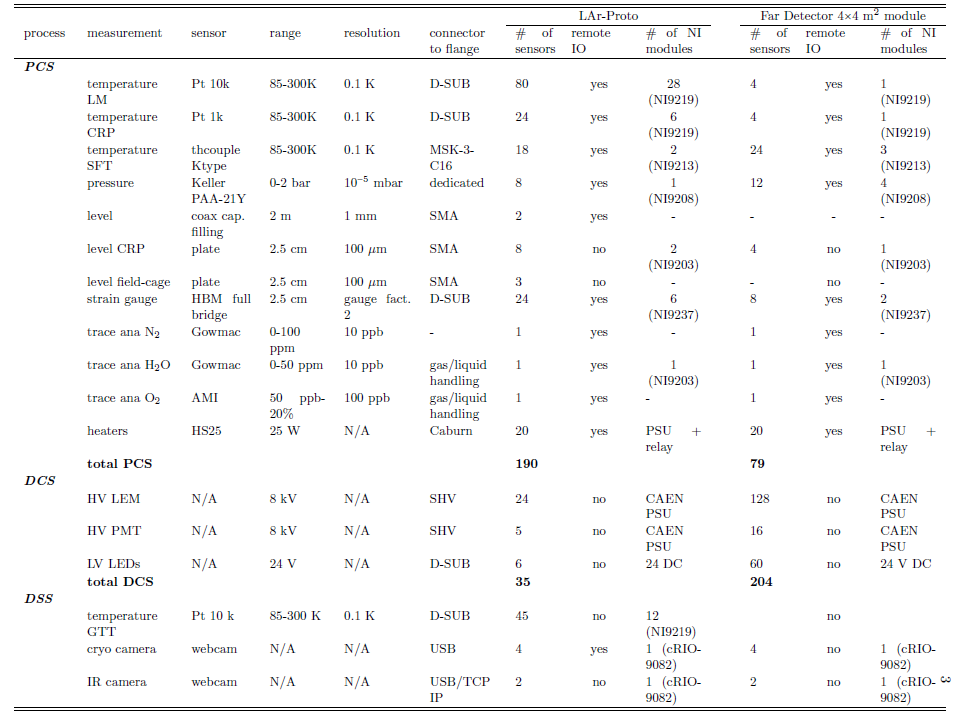
\includegraphics[scale=0.6, angle=0]{sc_table.png} %[scale=0.52, angle=0]{sc_table.png}
 \end{cdrfigure}
   